\documentclass{article}
\usepackage[utf8]{inputenc}
\usepackage{graphicx}
\usepackage[portuguese]{babel}
\usepackage{natbib}



\title{IF682- Engenharia de Software e Sistemas}
\author{Túlio Nolêto Caldas - tnc}
\date {Dezembro 2021}


\begin{document}




\maketitle

\paragraph{}

\section{\textbf{Introdução}}

{ Engenharia de Software náo é apenas sobre desenvolver softwares em si. Ocorrem processos envolvidos que resultam numa obtenção de um produto de software, que passa pelos processos de: desenvolvimento,definição, planejamento, e manutenção.
Logo, a cadeira não é restrita a "codar", uma atividade que pode ser desenvolvida de forma independente de outras pessoas, mas de atividades que requerem trabalho em equipe e capacidade de comunicação. Nesta ccadeita, são estudados princípios da Engenharia de Software, tais eles que serão discutidos posteriormente neste trabalho.}\cite{Intro}

\paragraph{}


\begin{figure}[h!]
\centering
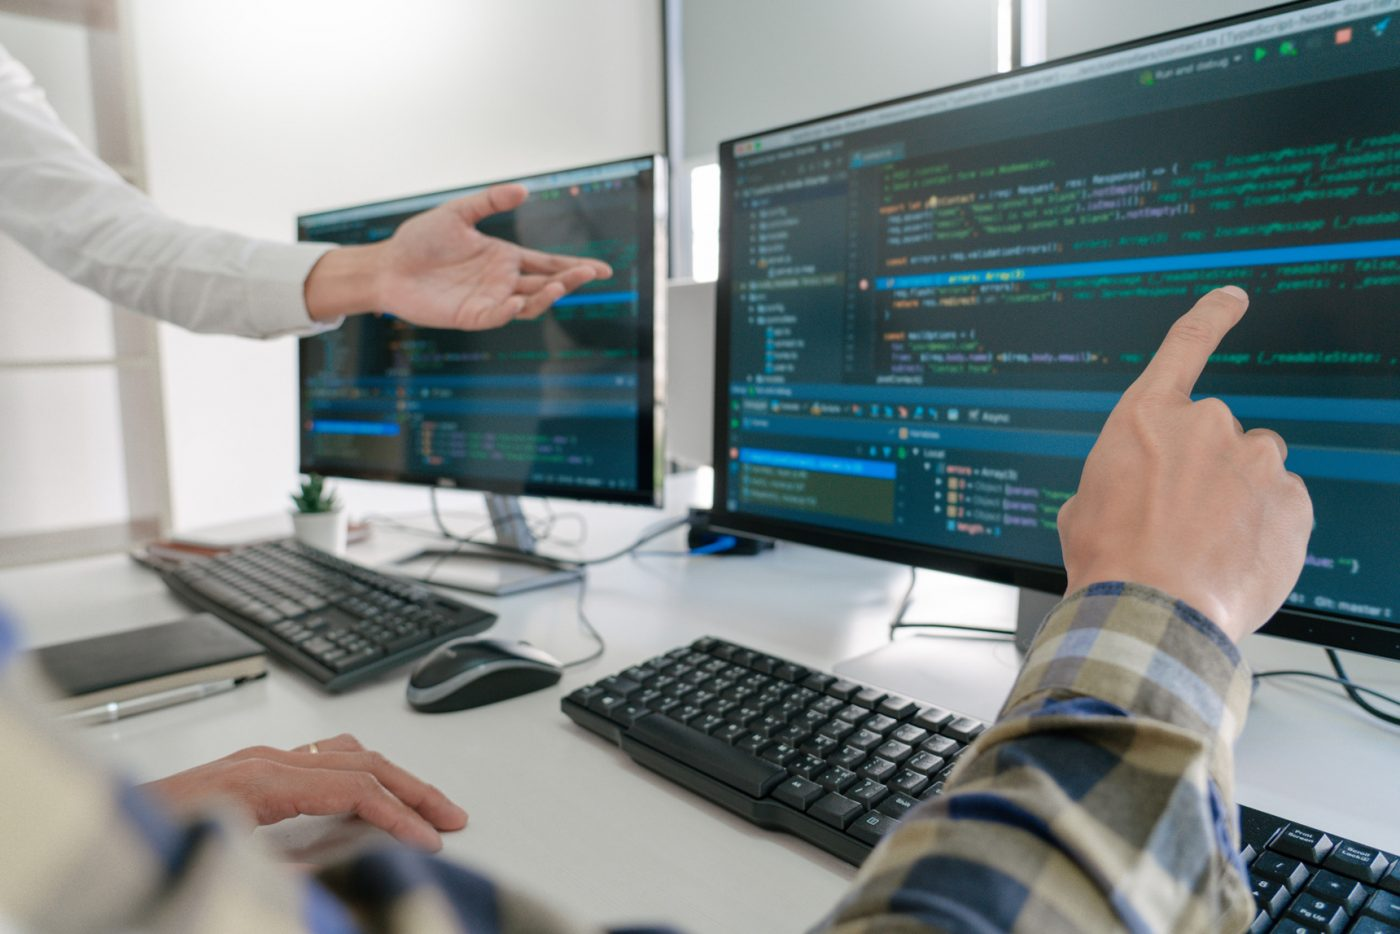
\includegraphics[scale=0.18]{imagens/Computador.jpeg} 
\caption{Imagem representando desenvolvimento de softwares e sistemas}\cite{computador1}
\label{fig:computador}
\end{figure}

  

\vspace{2 cm}


\section{Definições}
{ A Engenharia de Software e Sistemas em si, pode ser caracterizada como uma metodologia de manutenção e desenvolvimento de sistemas modulares. Alguns deles são:}\cite{rezende2006engenharia}
\begin{itemize}
    \item Planejamento e gestão de recursos e atividades
    \item Fundamentação na tecnologia da informação
    \item Adequação aos requisitos dos clientela e seus procedimentos 
    \item Padrão de qualidade para com o seus proddutos e atividades
    \item Processo de soluções eficazes e dinâmicas de soluções tencológicas
\end{itemize}

\vspace{2 cm}

\section{Objetivos}
{ O objetivo principal deste curso é estudar, analisar, discutir, e aplicar conceitos de Engenharia de Software. Do ponto de vista prático, os conceitos estudados serão aplicados no desenvolvimento de um projeto de software.}\cite{Objetivos}

{A ementa oficial da disciplina é a seguinte:}

\begin{itemize}
    \item Planejamento e Gerenciamento de Software
    \item Requisitos de Software
    \item Análise e Projeto de Software
    \item Codificação de Software
    \item Depuração e Testes
\end{itemize}

\vspace{2 cm}

\section{Relação}
{Para se cursar tal cadeira é necessário como pré-requisito deve antes pagar as respectivas cadeiras:}\cite{relacao}
\begin{itemize}
    \item Algoritmos e Estrutura de Dados - IF672
    \item Lógica para Computação - IF673
    \item[*] Equivalente á cadeira : Engenharia de Software - IF570
\end{itemize}


\vspace{2 cm}

\section{Relevância}
{A cadeira possui importância ímpar para o desenvolvimento do aluno como futuro profissional e sua entrada no mercado de trabalho, ajudando a desenvolver sistemas softwares, além de desenvolver o relacionamento e gerenciamento para com as pessoas}

\vspace{2 cm}

\bibliographystyle{plain}
\bibliography{ref}

\end{document}
